!TeX root = BasiDiDati.tex

\chapter{Laboratorio}
PostgrSQL è un Relational Data Base Management System (RDBMS o DBMS) con alcune funzionalità orientate agli oggetti. L’interazione tra un utente (programmatore/utente finale) e le basi di dati gestite da PostgreSQL avviene secondo il modello client-server.

    \begin{figure}[H]
      \centering
      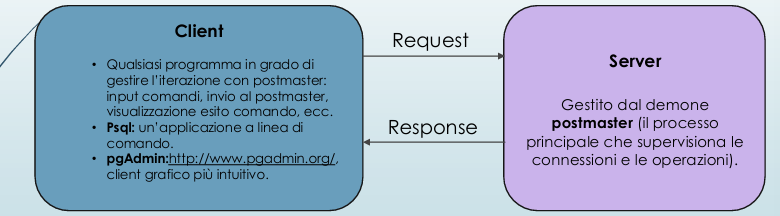
\includegraphics[width= \textwidth]{images/ClientServer.png}
    \end{figure}

    \section{Creazione di una tabella}
Struttura base
\begin{codiceSQL}
CREATE TABLE tabella (
  attributo dominio [ valoreDefault ] { vincolo }
  {, attributo dominio [ valoreDefault ] { vincolo } }
  {, vincoloTabella }
]);
\end{codiceSQL}

Costrutti inseriti: 
\begin{itemize}
  \item {[}{]} indicano parti opzionali / facoltative (il termine può non comparire o comparire una sola volta) Indica che quell'elemento può apparire zero o una volta. Sta al programmatore decidere se inserirlo o meno a seconda di ciò che si vuole ottenere)
\item {[} valoreDefault {]}: Significa che quando definisco l’attributo posso decidere se attribuirgli un valore predefinito
\item \{ \} Tutto ciò che è racchiuso tra parentesi graffe rappresenta un elemento che può essere ripetuto zero, una o più volte.
\item \{ vincolo \}: Significa che a una singola colonna puoi applicare nessun vincolo, un solo vincolo, oppure una serie di vincoli uno dopo l'altro (es. NOT NULL, UNIQUE)
\end{itemize}


\textbf{\large Ecco un esempio}
\begin{codiceSQL}
CREATE TABLE Impiegato (
  Matricola CHARACTER(6) PRIMARY KEY, 
  Nome VARCHAR(20) NOT NULL, 
  Cognome VARCHAR(20) NOT NULL,
  Dipart VARCHAR(15), 
  Stipendio NUMERIC(9) DEFAULT 0,
  FOREIGN KEY(Dipart) 
    REFERENCES Dipartimento(NomeDip),     /*vincolo di tabella*/
  UNIQUE (Cognome,Nome)                   /*vincolo di tabella*/
)
\end{codiceSQL}


\subsection{Identificatori}
 Sono stringhe che iniziano con una lettera (UTF-8) o un underscore (\_) e che possono contenere anche cifre (0-9). Gli identificatori SQL \textbf{NON} sono sensibili al minuscolo/maiuscolo:
 \begin{itemize}
  \item idPersona e idpersona rappresentano un solo identificatore.
 \end{itemize}

\subsection{Domini}
I domini elementari (predefiniti) sono:
\begin{itemize}
  \item \textbf{caratteri}: singoli caratteri o stringhe anche di lunghezza variabile
  \item \textbf{bit}: bit singoli (booleani) o stringhe di bit
  \item \textbf{numerici esatti e approssimati}
  \item \textbf{istanti temporali}
  \item \textbf{intervalli temporali}
\end{itemize}
Oppure si possono avere domini definiti dall'utente

\subsubsection{Tipo carattere}
Permette di rappresentare singoli caratteri oppure stringhe.
Un carattere o stringa di caratteri sono rappresentati tra apici (’):
’a’, ’Questa è una stringa’.\par
La lunghezza delle stringhe può essere fissa o variabile: 
\textcolor{cyan}{CHARACTER [VARYING][(lunghezza)]}
\begin{itemize}
  \item \textbf{CHARACTER}: carattere singolo
  \item \textbf{CHARACTER(20)}: stringa di \textbf{lunghezza fissa}. Se si assegna una stringa di lunghezza inferiore a 20, la stringa viene riempita di spazi fino a rendere la stringa lunga 20.
  \item \textbf{CHARACTER VARYING(20)}: stringa di \textbf{lunghezza variabile} (max 20).
  \item \textbf{TEXT}: \underline{stringa di lunghezza variabile senza limite fissato}. Questa è un’estensione PostgreSQL
\end{itemize}

\subsubsection{Tipo boolean}
Permette di rappresentare i valori booleani TRUE/FALSE, rappresentati anche 
come t/f, 1/0, yes/NO, più lo stato unknown (valore nullo), rappresentato 
come NULL

\subsubsection{Tipo numerici esatti}
Permettono di rappresentare valori esatti: interi o con una parte decimale di 
lunghezza prefissata
\begin{itemize}
  \item \textbf{Valori interi}:
\begin{itemize}
  \item SMALLINT: valori interi (2 bytes: da -32.768 (215) a +32.767 (215-1)).
  \item INTEGER: valori interi (4 bytes: da -2147483648 (231) to +2147483647 (231-1) ).
\end{itemize}
\item \textbf{Valori decimali}:
\begin{itemize}
  \item NUMERIC [(precisione [, scala])]: precisione è il numero totale di cifre  significative (cioè di cifre a sinistra e a destra della virgola), scala è il numero di cifre dopo la virgola (vuoto = 0).
\item DECIMAL [(precisione [, scala])]: equivalente al precedente.
\end{itemize}
\end{itemize}

\esempio{}{NUMERIC(5,2) permette di rappresentare valori come 100.01, 100.999 
(arrotondato a 101.00), ma non valori come 1000.01}

\subsubsection{Tipo numerici approssimati}
Permettono di rappresentare valori in virgola mobile:
\begin{itemize}
  \item \textbf{REAL}: una precisione di 6 cifre decimali.
  \item \textbf{DOUBLE PRECISION}: una precisione di 15 cifre decimali.
\end{itemize}
Ciascun numero è rappresentato da una coppia di valori: la mantissa e 
l’esponente.
\begin{itemize}
  \item La mantissa è un numero frazionario, l’esponente è un numero intero
  \item Il valore si ottiene moltiplicando la mantissa per la potenza di 10 con grado pari all’esponente
\end{itemize}
Il numero 0.17E16 corrisponde a 1,7 x 1015           
Il numero -0.4E-6 corrisponde a -4 x 10-7

\subsubsection{Istanti temporali}
Permettono di rappresentare istanti di tempo.
\begin{itemize}
  \item \textbf{DATE}: istanti del tipo (anno, mese, giorno).
  \begin{itemize}
    \item Un valore DATE si rappresenta tra apici (’) e lo standard ISO prescrive il formato \texttt{YYYY-MM-DD}.
  \end{itemize}
  \item \textbf{TIME [(precisione)][WITH TIME ZONE]}: istanti del tipo (hour, minute, second)
  \begin{itemize}
    \item precisione: numero cifre decimali per rappresentare frazioni del secondo;
    \item WITH TIME ZONE: permette di specificare anche [+-]hour:minute, che rappresentano la differenza con l’ora di Greenwich, o nomeFusoOrario.
  \end{itemize}
  \item \textbf{TIMESTAMP [(precisione)][WITH TIME ZONE]}: date + time.
\end{itemize}

\subsubsection{Intervalli temporali}
INTERVAL PrimaUnitàDiTempo[TO UltimaUnitàDiTempo]
PrimaUnitàDiTempoe UltimaUnitàDiTempodefiniscono le unità di misura che 
devono essere utilizzate, dalla più precisa alla meno precisa.
L’insieme delle unità di misura è diviso in due insiemi distinti:
\begin{itemize}
  \item Year-Month
  \item Day-Hour–Minute-Second
\end{itemize}

\subsubsection{Domini definiti dall'utente}

\begin{codiceSQL}
  CREATE DOMAIN nome AS tipoBase [valoreDefault][vincolo]
\end{codiceSQL}


\textcolor{purple}{\textbf{CREATE DOMAIN}}: definisce un dominio, utilizzabile in definizioni di relazioni, anche con 
vincoli e valori di default
Il dominio può essere definito a partire da un dominio elementare oppure da un altro 
dominio definito dall‘utente
\begin{codiceSQL}
CREATE DOMAIN giorniSettimana AS CHARACTER (3)
CHECK (VALUE IN ('LUN', 'MAR', 'MER', 'GIO', 'VEN', 'SAB', 'DOM'));
\end{codiceSQL}

\begin{codiceSQL}
CREATE DOMAIN Voto AS SMALLINT DEFAULT NULL
CHECK ( value >=18 AND value <= 30 )
\end{codiceSQL}




\subsection{Vincoli intrarelazionali}

\begin{itemize}
  \item \textbf{NOT NULL}: il valore nullo non è ammesso per l'attributo, quindi il valore deve sempre essere specificato, o si assegna un valore di default
  \item \textbf{UNIQUE}: definisce (super)chiavi
  \begin{codiceSQL}
Nome VARCHAR(20),
Cognome VARCHAR(20),
UNIQUE(Nome,Cognome)

/* impone che non ci siano due righe che abbiano uguale sia il nome che il cognome*/
  \end{codiceSQL}

  \begin{codiceSQL}
Nome VARCHAR(20) UNIQUE,
Cognome VARCHAR(20) UNIQUE

/* impone che non ci siano due righe che abbiano lo stesso nome o lo stesso cognome*/ 
  \end{codiceSQL}
  \item \textbf{PRIMARY KEY}: chiave primaria (una sola, implica NOT NULL) 
  \begin{codiceSQL}
matricola CHAR (6) PRIMARY KEY;
/* se unico componente della chiave primaria*/
  \end{codiceSQL}

  \begin{codiceSQL}
nome VARCHAR(20),
cognome VARCHAR(20),
PRIMARY KEY(nome, cognome)

/* Se la chiave primaria ha piu attributi */
  \end{codiceSQL}
  \item \textbf{CHECK}: specifica un vincolo generico che deve soddisfare le tuple della tabella. Viene soddisfatto se la sua espressione è vera o nulla.
  
\begin{codiceSQL}
CREATE TABLE Impiegato (
  matricola CHAR(6) PRIMARY KEY,
  nome VARCHAR(20) NOT NULL,
  cognome VARCHAR(20) NOT NULL,
  qualifica VARCHAR(20),
  stipendio NUMERIC(8,2) DEFAULT 500.00 NOT NULL
  CHECK( stipendio >= 0.0 ),    /* check di attributo */
  UNIQUE( cognome, nome ),
  CHECK( nome <> cognome )      /* check di tabella */
)
  \end{codiceSQL}

\end{itemize}

\subsection{Vincoli interrelazionali}
Un vincolo di integrità referenziale (= interrelazionale) crea un legame tra i 
valori di un attributo (o di un insieme di attributi) A della tabella corrente (detta interna/slave) e i valori di un attributo (o di un insieme di attributi) B di un’altra tabella (detta esterna/master):
\begin{itemize}
  \item Impone che, in ogni tupla della tabella interna, il valore di A, se diverso dal valore nullo, sia presente tra i valori di B nella tabella esterna.
  \item  L’attributo B della tabella esterna deve essere soggetto a un vincolo 
UNIQUE (o PRIMARY KEY).
\end{itemize}
\vario{Nota:}{L’attributo (o insieme di attributi) B può anche non essere la 
chiave primaria, ma deve essere identificante per le tuple della tabella 
esterna}

\textbf{REFERENCES e FOREIGN KEY permettono di definire vincoli di integrità referenziale}

Per singoli attributi, basta utilizzare il costrutto \textcolor{purple}{\textbf{REFERENCES}}
\begin{codiceSQL}
CREATE TABLE Impiegato (
  Matricola CHARACTER(6) primary key,
  Nome CHARACTER VARYING(20)  not null,
  Cognome CHARACTER VARYING(20)  not null,
  Dipart CHARACTER VARYING(15) 
  REFERENCES Dipartimento(NomeDip),   
  /* Attributo chiave (singolo) di tabella esterna*/
  Ufficio NUMERIC(3),
  Stipendio  NUMERIC(9) default 0,
  UNIQUE (Cognome, Nome)
)
\end{codiceSQL}

Per attributi multipli, si usa il costrutto \textcolor{purple}{\textbf{FOREIGN KEY}} alla fine della definizione degli attributi, seguito da \textcolor{purple}{\textbf{REFERENCES}}
\begin{codiceSQL}
CREATE TABLE Impiegato (
  Matricola CHARACTER(6) primary key,
  Nome CHARACTER VARYING(20)  not null,
  Cognome CHARACTER VARYING(20)  not null,
  Dipart CHARACTER VARYING(15),
  REFERENCES Dipartimento(NomeDip),   
  Ufficio NUMERIC(3),
  Stipendio  NUMERIC(9) default 0,
  FOREIGN KEY(Nome, Cognome)
    REFERENCES Anagrafica (Nome, Cognome) 
    /* Tabella esterna con attributi chiave*/
)
\end{codiceSQL}

Vediamo un esempio più concreto:

\begin{figure}[H]
  \centering
  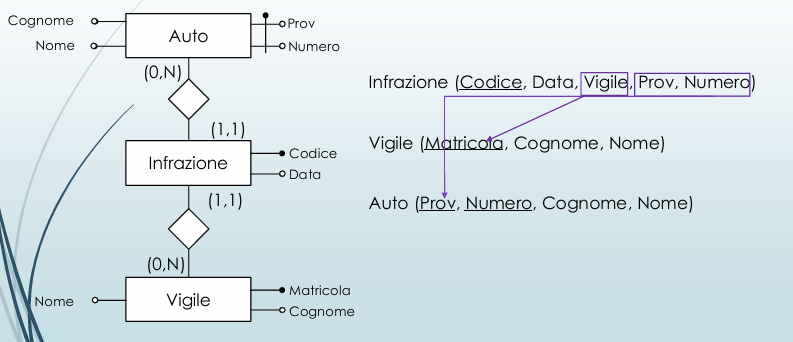
\includegraphics[width= \textwidth]{images/esempioReferences.png}
\end{figure}

\begin{codiceSQL}
CREATE TABLE Infrazione(
  Codice CHAR(6) PRIMARY KEY, 
  Data DATE NOT NULL,  
  Vigile INTEGER NOT NULL
  REFERENCES Vigile(Matricola),
  Provincia CHAR(2),  
  Numero CHAR(6) ,
  FOREIGN KEY(Provincia, Numero)
    REFERENCES Auto(Provincia, Numero)
)

\end{codiceSQL}

\section{Modifica degli schemi}
\begin{itemize}
  \item ALTER: effettua modifiche (a domini, tabelle...), ad esempio aggiungere una colonna a una relazione
  \item DROP DOMAIN: permette di rimuovere i domini
  \item DROP TABLE: cancella una tabella
\end{itemize}

\subsection{ALTER: modifiche alla struttura di una tabella}
Il costrutto \textbf{Alter} permette di:

Aggiungere un nuovo attributo (ADD COLUMN):
\begin{codiceSQL}
ALTER TABLE tabella ADD COLUMN attributo tipo;
ALTER TABLE impiegato ADD COLUMN stipendio NUMERIC(8,2);
\end{codiceSQL}

Rimuovere un attributo (DROP COLUMN):
\begin{codiceSQL}
ALTER TABLE tabella DROP COLUMN attributo;
ALTER TABLE impiegato DROP COLUMN stipendio;
\end{codiceSQL}
Modificare valore di default di un attributo (ALTER COLUMN):
\begin{codiceSQL}
ALTER TABLE tabella ALTER COLUMN attributo { SET DEFAULT valore | 
DROP DEFAULT };
ALTER TABLE impiegato ALTER COLUMN stipendio SET DEFAULT 1000.00;
\end{codiceSQL}

\section{Cancellazione dati in una tabella}
Le tuple di una tabella vengono cancellate con il comando \textcolor{purple}{\textbf{DELETE}}.
condizione è una espressione booleana che seleziona quali tuple cancellare. 
\begin{codiceSQL}
  DELETE FROM tabella [ WHERE condizione ];
\end{codiceSQL}

\vario{}{
  \textbf{Se WHERE non è presente, tutte le tuple saranno cancellate.}
}
\begin{codiceSQL}
  DELETE FROM impiegato WHERE matricola = 'A001 ';
\end{codiceSQL}

Una tabella viene cancellata con il comando \textcolor{purple}{\textbf{DROP TABLE}}:
\begin{codiceSQL}
  DROP TABLE tabella;
\end{codiceSQL}




\section{Inserimento e aggiornamento di tuple}

\textbf{\large Inserimento di valori all'interno di una tupla}

\begin{codiceSQL}
INSERT INTO Tabella [ ( Attributi ) ] 
VALUES( Valori ) 
\end{codiceSQL}
oppure
\begin{codiceSQL}
  INSERT INTO Tabella [ ( Attributi )]
(SELECT ...)
\end{codiceSQL}

\textbf{ Esempio inserimento}
\begin{codiceSQL}
INSERT INTO Museo (nome, citta, indirizzo, numeroTelefono, giornoChiusura, prezzo)
VALUES('Arena', 'Verona', 'piazza Bra', '045 8003204', 'MARTEDI', 20) 

\end{codiceSQL}


\textbf{\large Aggiornamento di valori all'interno di una tupla}

\begin{codiceSQL}
UPDATE NomeTabella
  SET Attributo = < 
  Espressione |
  SELECT ... | 
  NULL | 
  DEFAULT >
  [ WHERE Condizione ]
\end{codiceSQL}

\textbf{Esempio}
\begin{codiceSQL}
UPDATE Museo SET sitoInternet = 'www.ciao.it' WHERE citta ='Verona'  
\end{codiceSQL}


\section{Selezione}

\textbf{\large Struttura base}

\begin{codiceSQL}
SELECT [ DISTINCT ]
[ * | expression [[ AS] output_name ] [, 
...] ]
FROM from_item [, ...] 
[ WHERE condition ]
[ GROUP BY grouping_element [, ...] ]
[ HAVING condition [, ...] ]
[ { UNION | INTERSECT | EXCEPT } [ DISTINCT
] other_select ]
[ ORDER BY expression [ ASC | DESC | USING 
operator ]]

\end{codiceSQL}


\subsection{Clausola SELECT}
\begin{codiceSQL}
SELECT [ DISTINCT ]
[{* | expression [[ AS] output_name ]} [, ...]]
\end{codiceSQL}
\begin{description}
  \item [\textbf{*}] è un’abbreviazione per indicare tutti gli attributi delle tabelle.
  \item [\textbf{expression}] è un’espressione che coinvolge gli attributi della tabella (può anche essere semplicemente il nome di un attributo).
  \item [\textbf{output\_name}] è il nome assegnato all’attributo che conterrà il risultato della valutazione dell’espressione expression nella relazione risultato.
  \item [\textbf{DISTINCT}:] se presente richiede l’eliminazione delle tuple duplicate.

\end{description}


L’esecuzione di una \textbf{SELECT} produce una relazione che:
\begin{itemize}
  \item ha come schema tutti gli attributi elencati nella clausola \textbf{SELECT};
  \item ha come contenuto tutte le tuple ottenute proiettando sugli attributi 
indicati nella \textbf{SELECT} provenienti dalle tabelle del \textbf{FROM} (prodotto 
cartesiano), limitate a quelle che soddisfano le eventuali condizioni 
specificate nelle clausole \textbf{WHERE}, \textbf{GROUP BY} e \textbf{HAVING}
\end{itemize}


\subsubsection{Target List}

\begin{minipage}[t]{0.39\textwidth}
   \begin{codiceSQL}
SELECT *
FROM Tabella
   \end{codiceSQL}
\end{minipage}
\hfill % Questo comando inserisce uno spazio flessibile che spinge le due minipage ai lati opposti
\begin{minipage}[t]{0.50\textwidth}
  \vspace{1em}
   Selezione di tutti gli attributi 
delle tabelle indicate nella 
clausola FROM
\end{minipage}

\begin{minipage}[t]{0.39\textwidth}
   \begin{codiceSQL}
SELECT Attributo1, Attributo2
FROM Tabella
   \end{codiceSQL}
\end{minipage}
\hfill % Questo comando inserisce uno spazio flessibile che spinge le due minipage ai lati opposti
\begin{minipage}[t]{0.50\textwidth}
  \vspace{1em}
   Selezione di tutti gli attributi 
delle tabelle indicate nella 
clausola FROM
\end{minipage}


\textbf{Esempio}



\begin{minipage}[t]{0.39\textwidth}
 \begin{codiceSQL}
SELECT Nome, Reddito
FROM Persone
WHERE Eta < 30
\end{codiceSQL}
\end{minipage}
\hfill % Questo comando inserisce uno spazio flessibile che spinge le due minipage ai lati opposti
\begin{minipage}[t]{0.50\textwidth}
\begin{figure}[H]
  \centering
  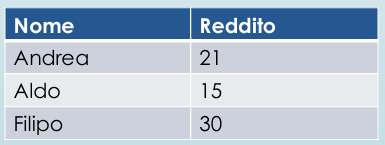
\includegraphics[width=\textwidth]{images/nomeReddito.png}
  \caption{selezionati solo le tuple dove è rispettata la condizione}
\end{figure}
\end{minipage}


\subsubsection{Concatenazione stringhe}
L'operatore di concatenazione || è un operatore scalare (o operatore di riga).

Lavora su una singola riga alla volta. Se la tua tabella ha 100 righe, il costrutto titolo || ' - ' || citta calcolerà e restituirà 100 risultati testuali separati, uno per ogni riga.

\vario{nota}{Non è un'esclusiva della SELECT}
può infatti essere utilizzato anche 

\textbf{\large Nella clausola WHERE (per filtrare i dati)}
\begin{codiceSQL}
  -- Trova la riga in cui l'unione di nome e cognome da esattamente 'Mario Rossi'
WHERE nome || ' ' || cognome = 'Mario Rossi'
\end{codiceSQL}

\textbf{\large Nella clausola ORDER BY (per ordinare i risultati)}
\begin{codiceSQL}
  -- Ordina i risultati basandosi sull'unione testuale dei due campi
ORDER BY titolo || citta
\end{codiceSQL}



\subsection{Clausola FROM}
\begin{codiceSQL}
  FROM from_item [, ...]
\end{codiceSQL}

\begin{enumerate}
  \item  table\_name [[AS] alias [(column\_alias [, ...])]]
  \begin{itemize}
    \item Se sono presenti due o più tabelle, si esegue il prodotto cartesiano tra tutte le  tabelle. Se ci sono attributi con lo stesso nome su tabelle diverse, nel SELECT 
questi attributi sono identificati anteponendo il nome della tabella e un ’.’: 
nomeTabella.nomeAttributo
  \end{itemize}

  \item  (other\_select) [AS] nomeRisultato [(column\_alias [,...])
  \begin{itemize}
    \item  è una SELECT innestata. Il risultato della SELECT interna è lo schema con nome 
nomeRisultato su cui fare la SELECT corrente.
  \end{itemize}

  \item  from\_item [NATURAL] join\_type from\_item [ON condition]
  \begin{itemize}
    \item  è la clausola JOIN.
    \item Metodo più sofisticato di 1) che permette di selezionare un sottoinsieme del 
prodotto cartesiano di due o più tabelle. join\_type specifica il tipo di join. I tipi 
principali sono riassunti nelle slide seguenti
  \end{itemize}
\end{enumerate}


\subsubsection{Uso di alias}

\begin{codiceSQL}
SELECT P.Reddito, R.Telefono
FROM Reparti as R, Persona ad P
WHERE ... ;
\end{codiceSQL}

Utile quando è necessario specificare la provenienza dell’attributo, 
perchè nella base di dati sono presenti più attributi con lo stesso nome

\subsubsection{Target List}
\begin{codiceSQL}
SELECT P.Nome as NPersona, P.Reddito as RPersona
FROM Persone as P
WHERE P.Eta < 30
\end{codiceSQL}




\subsection{Clausola WHERE}
\begin{codiceSQL}
  WHERE condition
\end{codiceSQL}

\textbf{\textcolor{black!50!red}{condition}} è un’espressione booleana combinando condizioni semplici $C_{i}$ con gli 
operatori AND, OR, NOT.
\begin{enumerate}
  \item  $C_{i}$ := expr [ $\theta$ \{expr | const\}]
dove
\begin{itemize}
  \item expr := espressione che contiene riferimenti agli attributi delle tabelle che compaiono 
nella clausola FROM.
\item $\theta \in$ \{=,<>,<,>,<=,>=\}
\item const := valore dei domini di base.
\end{itemize}
\item Una riga soddisfa \textcolor{black!50!red}{condition} se l’espressione è vera quando valutata con i valori 
della riga.
\item Una riga che non soddisfa condition è scartata dal risultato finale
\end{enumerate}





\begin{minipage}[t]{0.39\textwidth}
 \begin{codiceSQL}
SELECT Nome, Reddito
FROM Persone
WHERE Eta < 30;
\end{codiceSQL}
\end{minipage}
\hfill % Questo comando inserisce uno spazio flessibile che spinge le due minipage ai lati opposti
\begin{minipage}[t]{0.50\textwidth}
SELECT Nome, Reddito
FROM Persone
WHERE Età < 30 OR Reddito > 50;
\end{minipage}




\subsubsection{Operatore LIKE}
\begin{codiceSQL}
WHERE attributo [NOT] LIKE 'pattern';
\end{codiceSQL}

Nella clausola WHERE può apparire l’operatore LIKE per il confronto di stringhe. 
LIKE è un operatore di pattern matching. I pattern si costruiscono con i 
caratteri speciali \_ e \%:
\begin{itemize}
  \item \_ = 1 carattere qualsiasi.
  \item \% = 0 o più caratteri qualsiasi.
\end{itemize}


\begin{minipage}[t]{0.39\textwidth}
  \vspace{2em}
  \begin{codiceSQL}
SELECT Nome,Reddito
FROM Persona
WHERE Nome LIKE 'A\%a'
  \end{codiceSQL}
\end{minipage}
\hfill 
\begin{minipage}[t]{0.50\textwidth}
  \vspace{0pt}
  % Rimosso totalmente \begin{figure}[H] e \end{figure}
  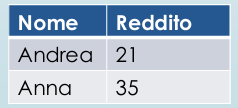
\includegraphics[width=0.8\textwidth]{images/nomeReddito2.png}
\end{minipage}  


\subsubsection{Operatore SIMILAR TO}


L’operatore \textbf{\textcolor{purple}{SIMILAR TO}} è un \textbf{\textcolor{purple}{LIKE}} più espressivo che accetta, come pattern, 
un sottoinsieme delle espressioni regolari POSIX (versione SQL). 
Esempi di componenti di espressioni regolari:
\begin{itemize}
  \item \_ = 1 carattere qualsiasi. 
  \item \% = 0 o più caratteri qualsiasi.
  \item * = ripetizione del precedente match 0 o più volte.
  \item + = ripetizione del precedente match UNA o più volte.
  \item \{n,m\} = ripetizione del precedente match almeno n e non più di m volte.
  \item {[} ... {]} = ... è un elenco di caratteri ammissibili
\end{itemize}


\begin{minipage}[t]{0.50\textwidth}
  \vspace*{0pt}
  \begin{codiceSQL}[unbreakable]
SELECT *
FROM Persone
WHERE Nome SIMILAR TO '[AFO]'
  \end{codiceSQL}
\end{minipage}
\hfill 
\begin{minipage}[t]{0.45\textwidth}
  \vspace*{0pt}
  \vspace{1.5em} % Spazio per allineare il testo al centro del codice
Per trovare nomi che inziano per A,F o O
\end{minipage}  


\subsubsection{Operatore BETWEEN}

\begin{codiceSQL}
WHERE attributo [NOT] BETWEEN valore_iniziale AND valore_finale;
\end{codiceSQL}

Nella clausola \textcolor{purple}{\textbf{WHERE}} può apparire l’operatore \textcolor{purple}{\textbf{BETWEEN}} per testare l’appartenenza 
di un valore ad un intervallo (non limitato ai valori numerici, usato anche con date e 
stringhe)


\begin{minipage}[t]{0.40\textwidth}
  \begin{codiceSQL} 
SELECT *
FROM Persone
WHERE Eta BETWEEN 20 AND 40
  \end{codiceSQL}
\end{minipage}
\hfill 
\begin{minipage}[t]{0.45\textwidth}
  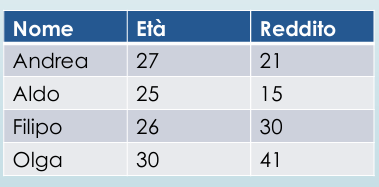
\includegraphics[width=0.8\textwidth, valign=t]{images/nomeEtaReddito.png}
\end{minipage}


\subsubsection{Operatore IN}
\begin{codiceSQL}
  WHERE attributo [NOT] IN ( valore [, ...] );

\end{codiceSQL}
Nella clausola WHERE può apparire l’operatore [\textbf{\textcolor{purple}{NOT}}] \textbf{\textcolor{purple}{IN}} per testare 
l’appartenenza di un valore ad un insieme.
\begin{codiceSQL}
SELECT *
FROM Persone
WHERE Nome NOT IN ('Andrea', 'Franco')
\end{codiceSQL}

\subsubsection{Operatore IS NULL}
\begin{codiceSQL}
WHERE attributo IS [ NOT ] NULL;
\end{codiceSQL}
Nella clausola WHERE può apparire l’operatore \textbf{\textcolor{purple}{IS}} [\textbf{\textcolor{purple}{NOT}}] \textbf{\textcolor{purple}{NULL}} per testare se un 
valore è \textbf{\textcolor{purple}{NOT KNOWN (NULL)}} o no.
Il valore NULL non rappresenta lo zero o una stringa vuota, ma l'assenza di dati 
o un valore sconosciuto.
A partire dalle versioni SQL-2 è stata adottata una logica a tre valori (true, 
false, unknown) e i valori nulli non sono considerati né veri, né falsi.\par
\begin{center}
NON SI PUÒ usare ’=’ o ’<>’ con il valore NULL!  
\end{center}

\begin{codiceSQL}
SELECT *
FROM Persone
WHERE Reddito IS NOT NULL
\end{codiceSQL}

\subsubsection{Operatore ORDER BY}
\begin{codiceSQL}
  ORDER BY attributo [{ ASC | DESC }] [, ... ];
\end{codiceSQL}
La clausola ORDER BY ordina le tuple del risultato in ordine rispetto agli attributi 
specificati,
ASCendente è lo standard.
\begin{codiceSQL}
SELECT Nome
FROM Persone
ORDER BY Nome DESC

\end{codiceSQL}

\subsubsection{Operatori di aggregazione}


Sono operatori che permettono di determinare un valore considerando i valori 
ottenuti da una SELECT.
Due tipi principali:
\begin{itemize}
  \item COUNT.
  \item MAX, MIN, AVG, SUM.
\end{itemize}

\begin{codiceSQL}
SELECT MAX(Reddito) 
FROM Persone;
\end{codiceSQL}

\vario{Nota}{Quando si usano gli operatori aggregati, dopo la SELECT non possono 
comparire espressioni che usano i valori presenti nelle singole tuple perché il 
risultato è sempre e solo una tupla
}



  \begin{enumerate}
    \item \textbf{Count}
    \begin{codiceSQL}
      COUNT({ *| expr | ALLexpr | DISTINCTexpr }])
    \end{codiceSQL}
    Restituisce il numero di tuple significative nel risultato dell’interrogazione.
    Tre casi comuni:\begin{itemize}
      \item \textcolor{purple}{COUNT(*)} ritorna il numero di tuple nel risultato dell’interrogazione.
      \item \textcolor{purple}{COUNT(expr)} ritorna il numero di tuple in ciascuna delle quali il valore expr è non nullo
      \item \textcolor{purple}{COUNT(ALL expr)} include duplicati e valori nulli.
      \item \textcolor{purple}{COUNT(DISTINCT expr)} come con \textcolor{purple}{COUNT(expr)} ma con l’ulteriore condizione che i valori di expr siano distinti
    \end{itemize}
    \item \textbf{SUM/MAX/MIN/AVG} 
    \begin{codiceSQL}
      op ({ expr | DISTINCTexpr })
    \end{codiceSQL}
    Determinano un valore numerico (SUM/AVG) o alfanumerico (MAX/MIN) considerando le tuple significative nel risultato dell’interrogazione.
    \begin{itemize}
      \item op = SUM | AVG | MAX | MIN;
      \item expr è un’espressione che usa uno o più attributi e funzioni di attributi.
      \item DISTINCT considero solo i valori distinti.  
    \end{itemize}
    \begin{codiceSQL}
      SELECT AVG(Eta) AS Media\_Eta
      FROM Persone;
    \end{codiceSQL}
  \end{enumerate}


  \section{Esempi di interrogazioni}
  \subsection{Interrogazione con raggruppamento: Group by}

  Un raggruppamento è un insieme di tuple che hanno medesimi valori su uno o più attributi caratteristici del raggruppamento.\par
La clausola GROUP BY attr [, ...] permette di determinare tutti i raggruppamenti delle tuple della relazione risultato (tuple selezionate con la clausola WHERE) in funzione degli attributi dati.\par
In una interrogazione che usa GROUP BY, la clausola SELECT contiene solamente gli attributi (da 0 a tutti) utilizzati per il raggruppamento ed eventuali funzioni di aggregazione sugli altri attributi.


\textbf{\large Visualizzare tutte le città raggruppate della tabella Studente}
\begin{codiceSQL}
SELECT citta
FROM studente
GROUP BY citta
\end{codiceSQL}

\noindent
\begin{minipage}[t]{0.6\textwidth}
   \centering
   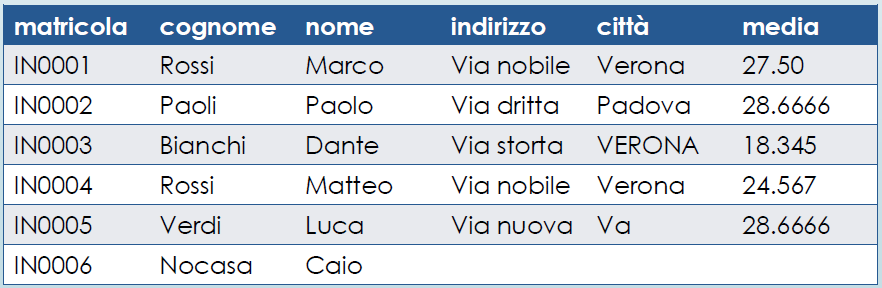
\includegraphics[width = 0.8\textwidth]{images/TableALL.png} 
\end{minipage}
\hfill % Questo comando inserisce uno spazio flessibile che spinge le due minipage ai lati opposti
\begin{minipage}[t]{0.38\textwidth}
   \centering
   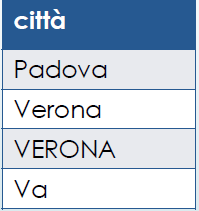
\includegraphics[width = 0.4\textwidth]{images/Group_By.png} 
\end{minipage}




\textbf{\large Visualizzare tutte le città e i cognomi raggruppati}




\noindent
\begin{minipage}{0.5\textwidth}
   \begin{codiceSQL}
SELECT cognome,LOWER(citta)
FROM Studente
GROUP BY cognome,LOWER(citta);
   \end{codiceSQL}
\end{minipage}
\hfill % Questo comando inserisce uno spazio flessibile che spinge le due minipage ai lati opposti
\begin{minipage}[t]{0.40\textwidth}
   \centering
   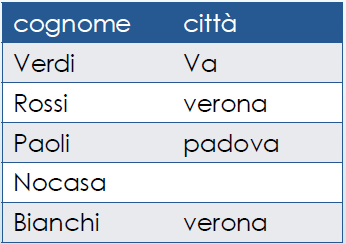
\includegraphics[width = 0.5\textwidth]{images/tabellaRisultante.png} 
\end{minipage}




\vario{Nota}{Nel GROUP BY non si possono usare espressioni con operatori di aggregazione.}

\vario{Nota}{Nella SELECT con GROUP BY non si possono specificare attributi che non sono raggruppati.}



\begin{itemize}
  \item La clausola WHERE permette di selezionare le righe che devono far parte del risultato.
  \item La clausola HAVING permette di selezionare i raggruppamenti che devono far parte del risultato.
  \item La sintassi è HAVING bool\_expr, dove bool\_expr è un’espressione booleana che può usare gli attributi usati nel GROUP BY e/o gli altri attributi mediante operatori di aggregazione.
\end{itemize}


\textbf{\large Visualizzare tutte le città raggruppate che iniziano con ’V’ della tabella Studente.}



\noindent
\begin{minipage}{0.5\textwidth}
   \begin{codiceSQL}
SELECT citta
FROM Studente
GROUP BY citta
HAVING citta LIKE 'V%';
   \end{codiceSQL}
\end{minipage}
\hfill % Questo comando inserisce uno spazio flessibile che spinge le due minipage ai lati opposti
\begin{minipage}[t]{0.40\textwidth}
   \centering
   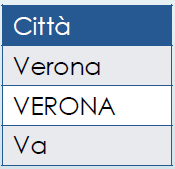
\includegraphics[width = 0.5\textwidth]{images/tabellaRisultante2.png} 
\end{minipage}




\textbf{\large Visualizzare tutte le città e i cognomi raggruppati con almeno due studenti con lo stesso cognome..}



\noindent
\begin{minipage}{0.5\textwidth}
   \begin{codiceSQL}
SELECT cognome, LOWER(citta)
FROM Studente
GROUP BY cognome, LOWER(citta)
HAVING COUNT ( cognome) >1;
   \end{codiceSQL}
\end{minipage}
\hfill % Questo comando inserisce uno spazio flessibile che spinge le due minipage ai lati opposti
\begin{minipage}[t]{0.40\textwidth}
   \centering
   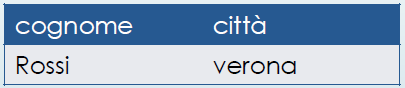
\includegraphics[width = 0.5\textwidth]{images/tabellaRisultante3.png} 
\end{minipage}



\textbf{\large Si possono specificare espressioni con operatori di aggregazione su attributi non raggruppati anche nella clausola HAVING.}



\noindent
\begin{minipage}{0.5\textwidth}
   \begin{codiceSQL}
SELECT LOWER(citta) AS "Citta", AVG (media)::DECIMAL(5 ,2) AS "mediaArr."
FROM Studente
GROUP BY LOWER(citta)
HAVING AVG(media) >23.47 ;
   \end{codiceSQL}
\end{minipage}
\hfill % Questo comando inserisce uno spazio flessibile che spinge le due minipage ai lati opposti
\begin{minipage}[t]{0.40\textwidth}
   \centering
   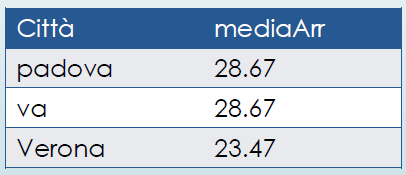
\includegraphics[width = 0.5\textwidth]{images/tabellaRisultante4.png} 
\end{minipage}



\subsection{Interrogazione con JOIN}

\begin{codiceSQL}
  TABLE1 join_typeTABLE2 ON join_condition[, ...].
\end{codiceSQL}


\textcolor{cyan}{INNER JOIN}, \textcolor{cyan}{LEFT [OUTER] JOIN}, \textcolor{cyan}{RIGHT [OUTER] JOIN} e \textcolor{cyan}{FULL [OUTER] JOIN}.
Dove \textcolor{cyan}{join\_condition} è un’espressione booleana che seleziona le tuple del join da aggiungere al risultato.
Le tuple selezionate possono essere poi filtrate con la condizione della clausola \textcolor{purple}{WHERE}.
Il prodotto cartesiano di due o più tabelle è un \textcolor{cyan}{CROSS JOIN}.


\textbf{\large Interrogazioni con INNER JOIN
Rappresenta}

\begin{codiceSQL}
  table1 [ INNER] JOIN table2 ON join_condition[, ...]
\end{codiceSQL}


Rappresenta il tradizionale $\theta$ join dell’algebra relazionale.
Combina ciascuna riga r1 di table1 con ciascuna riga di table2 che soddisfa la condizione della clausola ON.
table1 [ INNER] JOIN table2 ON join\_condition[, ...]



\subsection{Interrogazioni con LEFT OUTER JOIN}
\begin{codiceSQL}
  table1 LEFT[ OUTER] JOIN table2 ON join_condition[, ...].
\end{codiceSQL}

Si esegue un INNER JOIN. Poi, per ciascuna riga r1 di table1 che non soddisfa la condizione con qualsiasi riga di table2, si aggiunge una riga al risultato con i valori di r1 e assegnando NULL agli altri attributi..

Il LEFT [OUTER] JOIN non è simmetrico!
Con le medisime tabelle si possono ottenere risultati diversi invertendo l’ordine delle tabelle nel join!


\subsection{Interrogazioni con RIGHT OUTER JOIN}

\begin{codiceSQL}
  table1 RIGHT[ OUTER] JOIN table2 ON join_condition[, ...].
\end{codiceSQL}

Si esegue un INNER JOIN. Poi, per ciascuna riga r2 di table2 che non soddisfa la condizione con qualsiasi riga di table1, si aggiunge una riga al risultato con i valori di r2 e assegnando NULL agli altri attributi..


\subsection{Interrogazioni con FULL OUTER JOIN}

\begin{codiceSQL}
  table1 FULL[ OUTER] JOIN table2 ON join\_condition[, ...].
\end{codiceSQL}

\begin{itemize}
  \item È equivalentea:INNER JOIN + LEFT OUTER JOIN + RIGHT OUTER JOIN.
  \item \textcolor{black!60!red}{Non è equivalentea CROSS JOIN!}
\end{itemize}


  \section{Interrogazioni nidificate e insiemistiche}

  \subsection*{Interrogazioni nidificate}
  SQL permette la costruzione di interrogazioni che presentano al loro interno altre interrogazioni. 
La nidificazione può avvenire nelle clausole \textcolor{purple}{SELECT}, \textcolor{purple}{FROM}, \textcolor{purple}{WHERE}.
L'uso più comune è la nidificazione nella clausola WHERE

\subsection{Clausola FROM}
Con l'utilizzo di questa opzione, è possibile comporre catene di interrogazioni, 
in cui ciascuna interrogazione utilizza il risultato della precedente come se 
fosse una tabella di base

\begin{codiceSQL}
  SELECT titolo, prezzoIntero
FROM Mostra, ( SELECT MAX ( prezzoIntero ) 
FROM Mostra ) AS T( prezzoMax )
WHERE prezzoIntero = prezzoMax;
\end{codiceSQL}

\subsection{Clausola WHERE}
Il predicato (predicato complesso) nella clausola WHERE confronta un valore (ottenuto come espressione valutata sulla singola riga), con il risultato dell'esecuzione di un'interrogazione SQL (in generale un insieme di valori). 
Occorre estendere gli operatori di confronto per poter realizzare la comparazione tra un valore e un insieme di valori



Soluzione offerta da SQL: estensione degli operatori di confronto (>,<, =, <=, 
>=, <>) con ANY/SOME e ALL (IN, NOT IN). 
\begin{itemize}
  \item \textcolor{purple}{ANY/SOME}: specifica che la riga soddisfa la condizione se risulta vero il 
confronto (con l'operatore specificato) tra il valore dell'attributo per la riga e 
\textbf{almeno uno} degli elementi restituiti dall'interrogazione. 
  \item \textcolor{purple}{ALL}: specifica che la riga soddisfa la condizione solo se \textbf{tutti gli elementi} 
restituiti dall'interrogazione nidificata rendono vero il confronto. 
\item \textcolor{purple}{IN} e \textcolor{purple}{NOT IN}: usati per rappresentare l'appartenenza o l'esclusione rispetto ad 
un insieme (identici a = ANY o <>ALL)
\end{itemize}


\subsubsection{Operatore ANY/SOME}
\begin{codiceSQL}
  expression operator ANY( subquery )
expression operator SOME( subquery )
\end{codiceSQL}

\begin{itemize}
  \item \textcolor{orange}{expression} è un’espressione che coinvolge attributi della SELECT principale.
  \item (\textcolor{orange}{subquery}) è una \textcolor{purple}{SELECT} che deve restituire UNA sola colonna;
  \item \textcolor{orange}{operator} è un operatore di confronto, come ’=’, ’>=’, ...
  \item \textcolor{purple}{ANY} :è vero se la condizione è vera per almeno un valore della subquery.
  \item \textcolor{purple}{SOME} è uno sinonimo di \textcolor{purple}{ANY}
\end{itemize}


\textbf{\large Visualizzare il nome degli insegnamenti che hanno un numero di crediti 
inferiore alla media dell’ateneo di un qualsiasi anno accademico.}

\begin{codiceSQL}
  SELECT DISTINCT I.nomeins , IE.crediti
FROM Insegn I JOIN InsErogato IE ON I.id=IE.id_insegn
WHERE IE.crediti < ANY (
SELECT AVG ( crediti ) FROM InsErogato
WHERE modulo =0
GROUP BY annoaccademico
);
\end{codiceSQL}


\subsubsection{Operatore ALL}
\begin{codiceSQL}
  expression operator ALL( subquery )
\end{codiceSQL}

\begin{itemize}
  \item  \textcolor{orange}{expression} è un’espressione che coinvolge attributi della SELECT principale.
  \item (\textcolor{orange}{subquery}) è una \textcolor{purple}{SELECT} che deve restituire UNA sola colonna;
  \item \textcolor{orange}{operator} è un operatore di confronto, come ’=’, ’>=’, ...
  \item \textcolor{purple}{ALL}: La condizione è vera solo se è vera per TUTTI i valori della subquery.

\end{itemize}

\textbf{\large Trovare il nome degli insegnamenti con almeno un docente e crediti maggiori rispetto ai 
crediti di ciascun insegnamento del corso di laurea con id=6. (si considerano solo 
occorrenze insegnamento genitore)}

\begin{codiceSQL}
  SELECT DISTINCT I. nomeins , IE. crediti
FROM Insegn I JOIN InsErogato IE ON I.id = IE. id_insegn
JOIN Docenza D ON IE.id = D. id_inserogato
WHERE IE. modulo = 0 AND IE. crediti > ALL (
SELECT crediti FROM InsErogato
WHERE id_corsostudi = 6 AND modulo =0
);
\end{codiceSQL}

\subsubsection{Operatore IN}
E’ un operatore utilizzabile nei predicati complessi.
\begin{codiceSQL}
\[ROW\]( expr \[ ,...\]) IN ( subquery )  
\end{codiceSQL}
\begin{itemize}
  \item \textcolor{orange}{expr} è un’espressione costruita con un attributo della query principale. Ci 
possono essere una o più espressioni.
\item La (\textcolor{orange}{subquery}) deve restituire un numero di colonne pari al numero di 
espressioni in (\textcolor{orange}{expr} [,...]).
\item I valori dell’espressioni vengono confrontati con i valori di ciascuna riga del 
risultato di (subquery).
\item Il confronto ritorna vero se i valori sono uguali ai valori di almeno una riga della 
subquery.
\end{itemize}



\textbf{\large Trovare gli impiegati che hanno stesso nome e cognome di qualcuno in 
un’altra azienda.}
\begin{codiceSQL}
SELECT I.nome , I.cognome
FROMImpiegato I
WHERE ROW( I.nome , I.cognome ) IN (
SELECT I1.nome, I1. cognome FROM ImpiegatoAltraAzienda I1
)
\end{codiceSQL}



\subsubsection{Operatore EXIST}
E’ una clausola utilizzabile nei predicati complessi
\begin{codiceSQL}
  EXISTS(subquery)
\end{codiceSQL}


\begin{itemize}
  \item (subquery) è una \textcolor{purple}{SELECT}.
  \item \textcolor{purple}{EXISTS} ritorna falso se (subquery) non contiene righe; altrimenti vero.
  \item \textcolor{purple}{EXISTS} è significativo quando nella (subquery) si selezionano righe usando i 
valori della riga corrente nella \textcolor{purple}{SELECT} principale: \textcolor{red}{data binding. Vale a dire 
se subquery è un'interrogazione dipendente dalla query esterna}
\end{itemize}


\textbf{\large Determinare i nomi degli impiegati che sono diversi tra loro ma di pari 
lunghezza}

\begin{codiceSQL}
  SELECT I. nome
FROM Impiegato I
WHERE EXISTS (
SELECT 1 FROM Impiegato I1 WHERE I.nome <> I1. nome
AND CHAR_LENGTH( I.nome ) = CHAR_LENGTH( I1. nome )
)
\end{codiceSQL}
I.nome nella subquery è il valore di nome nella riga corrente della SELECT 
principale


\vario{Nota }{Se si usano attributi esterni nella subquery (data binding), la subquery
deve essere valutata per ogni riga della SELECT principale}


\textbf{\large Visualizzare il nome e il cognome dei docenti, escludendo i coordinatori, che hanno 
tenuto almeno due insegnamenti (o moduli) con più di 24 crediti nel 2010/2011}

\begin{codiceSQL}
  SELECT P.nome , P.cognome
FROM Persona P
WHERE EXISTS (
SELECT 1 FROM Docenza D JOIN InsErogato IE ON D. id_inserogato = IE.id
WHERE IE. crediti > 24 AND D. coordinatore = '0'
AND IE. annoaccademico = '2010/2011' AND D. id_persona = P.id
GROUP BY D. id_persona
HAVING COUNT (*) >=2
);

\end{codiceSQL}

\textbf{\large Visualizzare il nome dei corsi di studio che nel 2006/2007 non
hanno 
erogato insegnamenti il cui nome contiene la sottostringa ’Info’.}


\begin{codiceSQL}
  SELECT CS. nome FROM CorsoStudi CS
WHERE NOT EXISTS (
SELECT 1 FROM InsErogato IE JOIN Insegn I ON IE. id_insegn = 
I.id
WHERE I.nomeins LIKE '%Info%'
AND IE.annoaccademico = '2006/2007'
AND IE.id_corsostudi = CS.id)
\end{codiceSQL}



\subsection*{Interrogazioni di tipo insiemistico}

\begin{codiceSQL}
  query_1 { UNION | INTERSECT | EXCEPT } [ALL] query_2
\end{codiceSQL}

SQL mette a disposizione anche degli operatori insiemistici UNION, INTERSECT e 
EXCEPT per manipolare i risultati di più query.
Gli operatori insiemistici si possono utilizzare solo al livello più esterno di una 
query, operando sul risultato di due o più clausole SELECT.
Si possono avere sequenze di UNION/INTERSECT/EXCEPT


Gli operatori si possono applicare solo quando \textcolor{cyan}{query1} e \textcolor{cyan}{query2} producono 
risultati con lo stesso numero di colonne e di tipo compatibile fra loro.
Tutti gli operatori eliminano i duplicati dal risultato a meno che ALL non sia 
stato specificato.
\begin{itemize}
  \item \textcolor{red}{UNION} aggiunge il risultato di \textcolor{cyan}{query2} a quello di \textcolor{cyan}{query1}.
  \item \textcolor{red}{INTERSECT} restituisce le righe che sono presenti sia nel risultato di \textcolor{cyan}{query1} sia in quello di \textcolor{cyan}{query2}
  \item \textcolor{red}{EXCEPT} restituisce le righe di \textcolor{cyan}{query1} che non sono presenti nel risultato di \textcolor{cyan}{query2}. In pratica esegue la differenza insiemistica


\end{itemize}


\textbf{\large Visualizzare i nomi degli insegnamenti e i nomi dei corsi di laurea 
che non iniziano per 'A' mantenendo i duplicati}

\begin{codiceSQL}
  SELECT nomeins
FROM Insegn
WHERE NOT nomeins LIKE 'A%'
UNION ALL
SELECT nome
FROM CorsoStudi
WHERE NOT nome LIKE 'A%'
\end{codiceSQL}

    
\textbf{\large
  Visualizzare i nomi degli insegnamenti che sono anche nomi 
di corsi di laurea.
}

\begin{codiceSQL}
  SELECT nomeins
FROM Insegn
INTERSECT ALL
SELECT nome
FROM CorsoStudi;
\end{codiceSQL}

\textbf{\large Visualizzare i nomi degli insegnamenti che NON sono anche 
nomi di corsi di laurea.}

\begin{codiceSQL}
  SELECT nomeins
FROM Insegn
EXCEPT
SELECT nome
FROM CorsoStudi;
\end{codiceSQL}

\subsection{Le viste}

Le viste sono tabelle virtuali il cui contenuto dipende dal contenuto delle altre 
tabelle della base di dati.
In SQL le viste vengono definite associando un nome ed una lista di attributi al 
risultato dell’esecuzione di un’interrogazione.
\textcolor{purple}{Ogni volta che si usa una vista, si esegue la query che la definisce.}
Nell’interrogazione che definisce la vista possono comparire anche altre viste.
SQL \textcolor{red}{non ammette} però
\begin{itemize}
  \item  dipendenze immediate (definire una vista in termini di se stessa) o ricorsive 
(definire una interrogazione di base e una interrogazione ricorsiva);
\item dipendenze transitive circolari (V1 definita usando V2, V2 usando V3,. . . , Vn
usando V1).
\end{itemize}

\begin{codiceSQL}
  CREATE [ TEMP ] VIEW nome [( col_name [, ...]) ] AS query

\end{codiceSQL}

\textcolor{purple}{TEMP}: la vista è temporanea. Quando ci si sconnette, la vista viene distrutta. È 
un’estensione di PostgreSQL. Nella base di dati did2014 si possono fare solo 
viste temporanee

\begin{itemize}
  \item  \textcolor{cyan}{column\_name}: nomi delle colonne che compongono la vista; se non 
vengono specificati, sono ricavati dai nomi delle colonne restituiti dalla 
query, eventualmente tramite alias.
\item \textcolor{cyan}{query} deve restituire un insieme di attributi pari e nel medesimo ordine a 
quello specificato con ( \textcolor{cyan}{column\_name} [, ...] ) se presente.
\item SQL permette che una vista sia aggiornabile solo quando ciascuna tupla
della vista corrisponde a una sola tupla di ciascuna tabella di base.

\end{itemize}


\textbf{\large efinire la vista che contiene gli insegnamenti erogati completi di nomeins e codiceins
presi dalla tabella Insegn.}

\begin{codiceSQL}
  CREATE TEMP VIEW InsErogatiCompleti AS
SELECT I. nomeins , I. codiceins , IE .*
FROM InsErogato IE
JOIN Insegn I ON IE. id_insegn = I.id;
\end{codiceSQL}


\textbf{\large Si vuole determinare quali sono i corsi di studi con il massimo numero di nome di insegnamenti 
diversi}

Prima si crea una vista:
\begin{codiceSQL}
  CREATE TEMP VIEW InsCorsoStudi (Nome , NumIns) AS
SELECT CS.nome , COUNT ( DISTINCT I. nomeins )
FROM CorsoStudi CS
JOIN InsErogato IE ON CS.id=IE. id_corsostudi
JOIN Insegn I ON IE. id_insegn = I.id 
GROUP BY CS.nome;

\end{codiceSQL}

Poi la si usa:

\begin{codiceSQL}
  SELECT Nome, NumIns
FROM InsCorsoStudi
WHERE NumIns = ANY (
SELECT MAX ( NumIns ) FROM InsCorsoStudi);
\end{codiceSQL}

Laurea specialistica in Medicina e Chirurgia: 320


ora come dicevo marco succhia il bannano a tutti